\documentclass{beamer}
\usepackage{mathrsfs}  
\usepackage{xcolor}
\usepackage{setspace}
\usepackage{comment}
\usepackage[utf8]{inputenc}
\usepackage[T1]{fontenc}

% config du thgeme metropolis
\usetheme[progressbar=frametitle,block=fill, titleformat=smallcaps,sectionpage=progressbar,]{metropolis}



\title{Rappels : Analyse Univariée et Bivariée}
\subtitle{}
\date{2021-2022}
\author{Paul Chapron \textsuperscript{1} \& Yann Ménéroux \textsuperscript{1}}
\institute{ \textsuperscript{1}IGN-ENSG-UGE}



%definition de la couleur du texte dans la balise \alert{}
\definecolor{vertIGN}{HTML}{96C31E} % vert IGN %vrai valeur #97BE0D
\setbeamercolor{alerted text}{fg=vertIGN}

\definecolor{grisIGN}{HTML}{22292F} % Gris IGN tiré vers le noir 
\setbeamercolor{background canvas}{bg=grisIGN}




% code pour placer le log ENSG dans le bandeau de titre 
\makeatletter
\setbeamertemplate{frametitle}{%
  \nointerlineskip%
  \begin{beamercolorbox}[%
      wd=\paperwidth,%
      sep=0pt,%
      leftskip=\metropolis@frametitle@padding,%
      rightskip=\metropolis@frametitle@padding,%
    ]{frametitle}%
  \metropolis@frametitlestrut@start%
  \insertframetitle%
  \nolinebreak%
  \metropolis@frametitlestrut@end%
  \hfill
  \raisebox{-0.6ex}{\includegraphics[height=4ex,keepaspectratio]{img/logoENSG_small.jpg}}
  \end{beamercolorbox}%
}
\makeatother




% logo ENSG première page 
\titlegraphic{\vspace{4cm}\flushright\includegraphics[width=2cm,height=2cm]{img/logoENSG_big.png}} 



\begin{document}
\metroset{background=dark} % change background theme according to manual
\maketitle	

\section{Introduction} 

\begin{frame}{Dans les cours précédents ... }


Notions pour manipuler les \alert{variables aléatoires}, et estimer certains descripteurs

\begin{itemize}
\item co-variance
\item intervalle de confiance 
\item bootstrap
\item \dots
\end{itemize}

\end{frame}


\begin{frame}{Motivation}


L'analyse \alert{univariée} permet de \alert{décrire la forme}  et de \alert{quantifier} les caractéristiques de  la \alert{répartition des valeurs} d'une variable.



\begin{itemize}
	\item Notion de distribution 
	\item Visualisation ( Histogramme, densité, boxplots, \dots)
	\item Moments, Quantiles, CV 
\end{itemize}
\end{frame}






\section{Analyse Univariée}



\begin{frame}{Histogramme}

 \begin{block}{Histogramme d'une variable}
Représentation graphique des \alert{effectifs} associés à des \alert{classes de valeurs} d'une variable numérique 
\end{block}

Le nombre de classes peut varier ! 


\begin{figure}[!htb]
   \begin{minipage}{0.5\textwidth}
     \centering
     \includegraphics[width=.9\linewidth]{img/histogramme1.png}
     
   \end{minipage}\hfill
   \begin{minipage}{0.5\textwidth}
     \centering
     \includegraphics[width=.9\linewidth]{img/histogramme2.png}
     
   \end{minipage}
\end{figure}




\end{frame}


\begin{frame}{Distribution}

\begin{tiny}
  Synonymes: distribution empirique, distribution des fréquences, distribution statistique
\end{tiny}

\alert{Tableau} ou \alert{graphique} qui associe les (classes de) valeurs à leur \alert{fréquence d'apparition}


$\approx$ « Histogramme des fréquences en continu»


\begin{figure}
  \centering
     \includegraphics[width=.7\linewidth]{img/densité.png}
\end{figure}
\end{frame}

\begin{frame}{Distribution}





La distribution peut être définie comme une \alert{fonction} qui donne la probabilité qu’un individu $x$ pris au hasard  ait la valeur $V_x$ pour la variable $V$ : 

$$distribution(V) \equiv P(V=V_x),\forall V_x \in \Omega_V$$ 

Avec $\Omega_V$  l’ensemble des valeurs que peut prendre V : l’univers de V

Lorsque la variable prend des valeurs réelles, on parle de \alert{densité de probabilité}, c’est pourquoi on retrouve ce terme “density” sur les axes des ordonnées dans les graphiques de distribution.


\end{frame}

\begin{frame}{Distribution et histogramme}

\begin{figure}
  \centering
     \includegraphics[width=.7\linewidth]{img/histo_dens.png}
\end{figure}

\begin{small}
\begin{spacing}{0.75}
\alert{N.B.} En toute rigueur, représenter une courbe de distribution de probabilité par dessus un histogramme est impropre : il faudrait deux graphiques distincts, ou au moins deux axes des ordonnées: un pour l’histogramme, représentant un effectif, l’autre pour la distribution , représentant une probabilité 
\end{spacing}
\end{small}

\end{frame}





\begin{frame}{Distribution et lois}

Parfois , les distributions empiriques ressemblent à celles de lois de probabilités connues. 

$\rightarrow$ on peut alors  \alert{modéliser}  la  variable par une variable aléatoire de loi fixée

$\rightarrow$ les paramètres de cette loi doivent être déterminés (ajustement).


\end{frame}


\begin{frame}{Décrire une distribution}


La forme d'une distribution donne beaucoup d'informations  : 

\begin{small}
\begin{itemize}
  \setlength\itemsep{-0.0em}
  \begin{spacing}{0.7}
 \item \alert{"pics"} : valeurs les plus représentées dans la population 
 \item présence de \alert{valeurs extrêmes} : la courbe de la distribution est tirée à gauche ou à droite du graphique
 \item \alert{symétrie} : les individus se répartissent équitablement de part et d'autre du pic  
 \item \alert{aplatissement} : la population est plus ou moins resserrée, ou  autour de certaines valeurs 
 \item \dots
 \end{spacing}
\end{itemize}
\end{small}

\begin{figure}
  \centering
     \includegraphics[width=.65\linewidth]{img/densité.png}
\end{figure}



\end{frame}


\section{Décrire une distribution : mesures de \alert{tendance centrale}}

\begin{frame}{Tendance Centrale}


La tendance centrale est \alert{une} valeur qui \alert{résume} une série de valeurs (quantitative)

\vspace{1cm}


\begin{itemize}
  \item Moyenne
  \item Médiane 
  \item Mode
\end{itemize}


\end{frame}


\begin{frame}{Moyenne}


$$ \bar{x} = \frac{1}{n}\sum_{i=0}^{n} x_i$$


\begin{spacing}{0.9}
\begin{small}
Avantage  : chaque valeur compte  \\
Inconvénients : \\ 
\begin{itemize}
  \item sensibilité aux valeurs extrêmes 
  \item pas de signification sur les valeurs discrètes (e.g. 2.5 enfants par foyer)
\end{itemize}

Pour y remédier (parfois): \\
$\rightarrow$ exclure les outliers\\
$\rightarrow$ utiliser un autre estimateur (médiane)\\
$\rightarrow$ étudier la distribution des valeurs (e.g. cas bimodal) et opérer une classification
\end{small}
\end{spacing}

\end{frame}



\begin{frame}{Moyenne géométrique}

$$ \bar{x}_{geom} = \sqrt[n]{\prod _{i=0}^{n} x_i}$$  


Moins sensible que la moyenne classique aux valeurs extrêmes.

\end{frame}



\begin{frame}{Mode}


Le \alert{mode} d’une variable est la valeur la plus \alert{fréquente} ( d’effectif maximum) d’une variable.
\begin{spacing}{0.9}
\begin{small}
Avantages  : 
\begin{itemize}
  \item peu sensible aux valeurs extrêmes 
  \item interprétation  simple : cas le plus fréquent
\end{itemize}  
Inconvénient :  la valeur du mode ne dépend pas de toutes les observations, la modification d'une valeur n'entraîne pas la modification du mode (ce qui explique sa robustesse aux valeurs extrêmes)

\end{small}
\end{spacing}

\end{frame}



\begin{frame}{Calcul du mode}
Si la variable est quantitative et continue : 
\begin{itemize}
  \item découper l’étendue de la variable ($max -min$) en intervalle égaux
  \item compter les effectifs de chaque intervalle
  \item le mode est la moyenne des valeurs des bornes de l'intervalle de plus grand effectif.
\end{itemize}

\begin{tiny}
(C’est exactement ce que fait un histogramme graphiquement !)
\end{tiny}

\end{frame}



\begin{frame}{Modes}

Par définition, le mode est unique, mais on peut appeler modes les valeurs des autres pics d’une distribution.\\

 On parle de distribution \alert{bi-modale} ou \alert{tri-modale} lorsqu’une distribution présente deux ou trois pics. 

 Les \alert{valeurs modales} d’une distribution sont les valeurs correspondant à ces pics. 



\begin{figure}
  \centering
     \includegraphics[width=.7\linewidth]{img/trimodale.png}
\end{figure}

\end{frame}


\begin{frame}{Médiane}

La \alert{médiane} est la valeur qui sépare une population en \alert{deux} classes d'égal effectif.\\

C'est la valeur la plus proche de toutes les autres.


\begin{spacing}{0.9}
\begin{small}
Avantages  : 
\begin{itemize}
\item Souvent plus pertinente que la moyenne
\item les valeurs extrêmes ne modifient pas sa valeur
\item interprétation  facile: un individu sur deux a une valeur inférieure (respectivement supérieure) à la médiane.
\end{itemize}
\end{small}
\end{spacing}


Inconvénient : Comme le mode , la médiane ne dépend pas de toutes les observations 

\begin{tiny}
\begin{spacing}{0.9}
\alert{N.B.} la robustesse de la médiane est bien utile dans le cas de distribution particulièrement asymétriques, où la moyenne est dégradée par les valeurs extrêmes, à droite (valeurs très élevées) ou à gauche (valeurs très faibles).
\end{spacing}
\end{tiny}

\end{frame}




\begin{frame}{Moyenne et médiane}

Que peut on dire d'une population dont la médiane est inférieure à la moyenne ? 


Exemple : revenus mensuels en équivalent temps plein en France en 2016 : le revenu mensuel net moyen est de 2 238 €, le revenu mensuel net médian est de 1 789 € : selon l’\url{https://www.insee.fr/fr/statistiques/4277680?sommaire=4318291}

Supposons qu’on cherche à évaluer si un salaire mensuel net équivalent temps plein de 2000€ est un bon salaire en France, sans définir trop rigoureusement ce qui signifie «bon».

2000€ est inférieur à la moyenne du pays, on peut le considérer comme trop bas pour être «bon».
2000€ est supérieur au salaire médian, il est supérieur à (au moins) la moitié des salaires du pays, et on peut logiquement le considérer comme un «bon» salaire.
Cette double interprétation est due au fait que certains salaires très élevés, mais d’effectifs peu nombreux, tirent la distribution du salaire vers la droite, et avec eux, la moyenne.



\end{frame}



\begin{frame}{Moyenne et médiane}

Que peut on dire d'une population dont la médiane est inférieure à la moyenne ? 

\end{frame}




\section{Décrire une distribution : mesures de \alert{dispersion}}

\begin{frame}{Dispersion}


La tendance centrale est \alert{une} valeur qui \alert{résume} une série de valeurs (quantitative)


\end{frame}



\begin{comment}





\begin{columns}[T,onlytextwidth]
\column{0.48\textwidth}

\begin{itemize}

\item Plus la valeur $Contrib_{ik}$ est extrême, plus elle influe sur la direction de l'axe $k$
\item la coordonnée doit être rapportée à  l'étirement du nuage de points donné par  $\lambda_k$
\item filtrer des individus extrèmes \textit{peut} améliorer l'ACP ! 
\end{itemize}

\column{0.4\textwidth}
\metroset{block=fill}
\colorbox{white}{\includegraphics[width=0.85\textwidth,keepaspectratio]{img/contribution_indiv_axe.png}}

\vspace{0.5cm}

\colorbox{white}{\includegraphics[width=0.75\textwidth,keepaspectratio]{img/contribution_indiv_axe2.png}}

\end{columns}

\end{frame}





\begin{frame}{Qualité de représentation des individus}

La \alert{qualité de représentation} de l'individu $i$ à l'axe $k$ s'écrit : 
$$Qlt_{ik}=cos^2(\theta_{ik})= \frac{c_{ik}^2}{\|P_i\| ^2}$$



\begin{columns}[T,onlytextwidth]
\column{0.48\textwidth}

\colorbox{white}{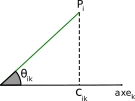
\includegraphics[width=0.85\textwidth,keepaspectratio]{img/angle_qualite_repres_axe.png}}

\column{0.48\textwidth}
\metroset{block=fill}

  Avec : 
  \begin{itemize}
  \setlength\itemsep{-0.1em}
  \item $c_{ik}$ la coordonnée de $i$ selon $k$
  \item $\theta_{ik}$ l'angle entre le vecteur $P_i$ et l'axe $k$
  \item $\|P_i\|$ la norme du vecteur  l'individu $i$
\end{itemize}
\end{columns}

\end{frame}



\begin{frame}{Bilan de l'ACP}


  \begin{columns}[T,onlytextwidth]
    \column{0.48\textwidth}
        \begin{alertblock}{Avantages}
        	\begin{itemize}
        		\item Réduit la dimensionnalité
        		\item Regroupe les variables et les individus 
            \item montre l'effet conjoint des variables 
        	\end{itemize}
      	\end{alertblock}

    \column{0.5\textwidth}
	\metroset{block=fill}
    
      \begin{block}{Limites}
        \begin{itemize}
            \item Composantes difficiles à interpréter en elles-mêmes
            \item hypothèses fortes : la  variance est un mélange "linéaire", et la  variance est de l'information, pas du bruit ($\approx$RSB fort)
            \item Que faire si $p$ est grand et si les premières composantes capturent peu d'inertie ?
        \end{itemize}
      \end{block}

      
  \end{columns}
\end{frame}




\begin{frame}{Pokémonologie}


\begin{columns}[T,onlytextwidth]
    \column{0.35\textwidth}

\includegraphics[width=\textwidth,keepaspectratio]{img/cercle_trigo_ACP_var.png}


  \column{0.65\textwidth}
\begin{small}  
\begin{itemize}
\item L'Axe 1 "prend tout" : c'est la puissance générale des pokémon, une sorte de \alert{score global}
\item L'Axe 2 sépare les variables en \alert{deux groupes} : celle du  combat "standard" (\texttt{Attack, Defense,HP}) et celles du combat "spécial/rapide" (\texttt{Sp..Atk, SP..Def, Speed})
\item On pourrait être tenté de diviser les pokemons en "Costauds classiques " vs. "Ninjas spéciaux" . 
\end{itemize}
\end{small}

\end{columns}

\medskip  
\medskip  \medskip  \medskip  \medskip  
\begin{tiny}
Merci à Anh Le , \url{https://anhqle.github.io/gotta-plot-them-all/}
\end{tiny}


\end{frame}



\begin{frame}{Références }


\begin{itemize}
\item \href{http://www.sthda.com/french/articles/38-methodes-des-composantes-principales-dans-r-guide-pratique/73-acp-analyse-en-composantes-principales-avec-r-l-essentiel}{\color{cyan}{Page ACP STDHA}}
\item \href{https://gitlab.huma-num.fr/hcommenges/cours_statcomplet}{\color{cyan}{Cours d'Hadrien Commenges}}
\end{itemize}


\end{frame}


\begin{comment}

\begin{frame}{Animation}
  \begin{itemize}[<+- | alert@+>]
    \item \alert<4>{This is\only<4>{ really} important}
    \item Now this
    \item And now this
  \end{itemize}
\end{frame}



\begin{frame}[standout]
Mono message sur une diapo
\end{frame}
\end{comment}

\end{document}